\documentclass{article}
\usepackage{amsmath}
\usepackage{MnSymbol}
\usepackage{wasysym}
\usepackage{graphicx}
\usepackage{float}

   \usepackage[numbered,framed]{matlab-prettifier}
\usepackage[export]{adjustbox}
\begin{document}
\begin{center}
\LARGE \bfseries{Answers to Problem Set 5}\\
 Group name: Ferienspass\vspace{.5cm}\\
 \normalsize \normalfont
  Sebastian K\"uhnl: 5642348\\
  Alexander D\"uck (as: reebyte): 5504077\\
  Patrick Blank (as: paddyblank): 6729110\\
  Christian Wierschem: 6729288
\end{center}
\normalsize	
\section{Question 1}
The approximate point where the household is indifferent between the two projects can be found via grid search. Graphically, the point where the two utility curves intersect in the point where the household becomes indifferent between the two projects. In both graphs, this point is marked by the vertical line going upwards from the horizontal line crossing through zero.
\begin{figure}[h]
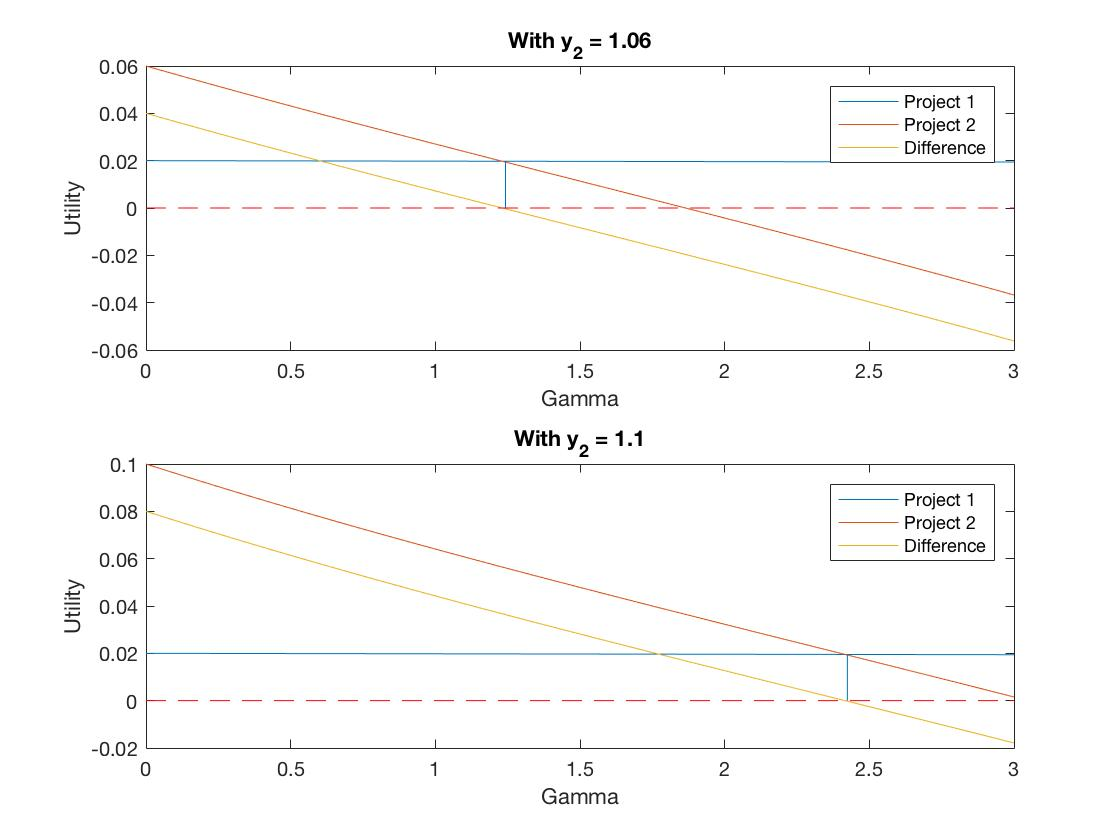
\includegraphics[width = \textwidth, keepaspectratio]{PS5Q2Sub3_Utility.jpg} 
\end{figure}
Alternatively, this point can also be found where the squared difference comes close to zero. \begin{figure}[h]
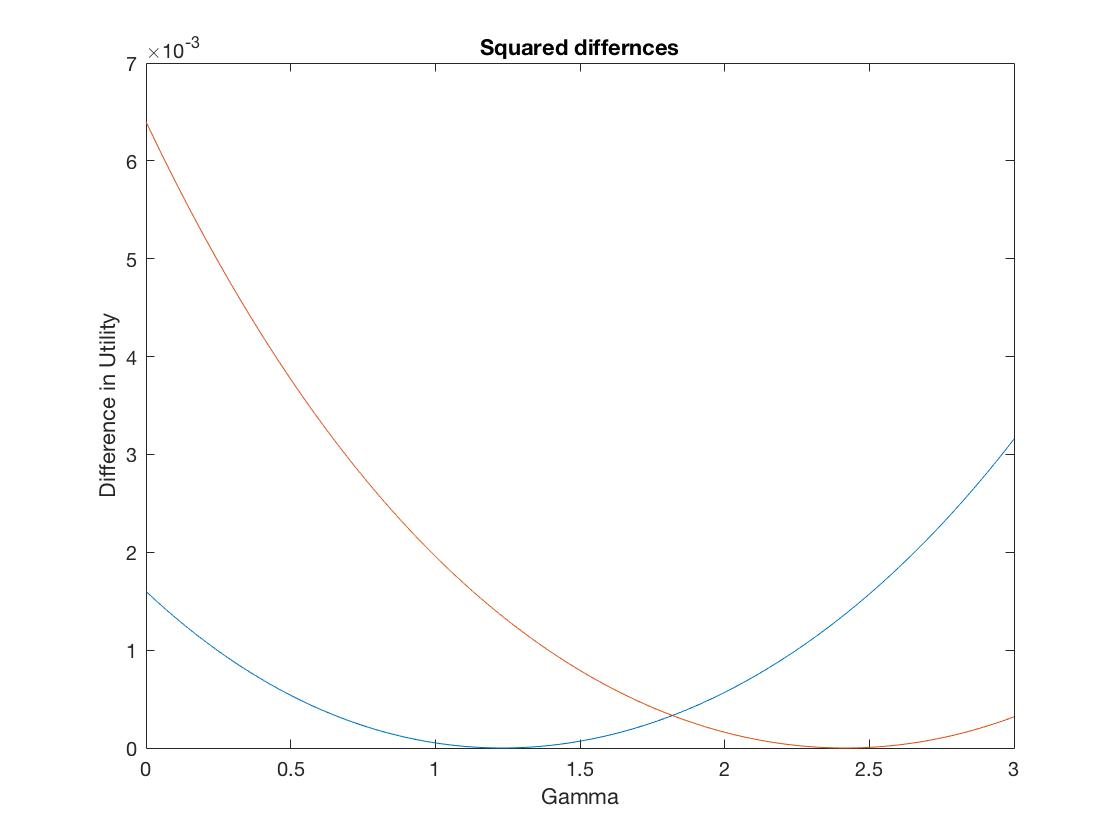
\includegraphics[width = \textwidth, keepaspectratio]{PS5Q2Sub3_Squared_Diff.jpg}
\end{figure}
However, for a truly satisfying result, grid search is not sufficient. The root of the difference function has to be found numerically. Here, the Newton algorithm is applied. For this, the first derivative with respect to $\gamma$ has to be computed. Since this is possible analytically, the derivation is provided below.
\begin{align}
u(c_t) &= \frac{c_t^{1-\gamma}-1}{1- \gamma} = \frac{c_t^{1-\gamma}}{1- \gamma} -\frac{1}{1- \gamma}\\
&= \frac{e^{(1-\gamma) \ln (c_t)}}{1- \gamma} -\frac{1}{1- \gamma}
\end{align}
The first derivative with respect to $\gamma$ can then be calculated:
\begin{align}
\frac{ \partial u(c_t)}{\partial \gamma} &= \frac{(-1)e^{(1-\gamma) \ln (c_t)} (1- \gamma)- (-1)e^{(1-\gamma) \ln (c_t)}}{(1- \gamma)^2} - \frac{0 - (-1)*1}{(1- \gamma)^2} \\
&= \frac{e^{(1-\gamma) \ln (c_t)}-e^{(1-\gamma) \ln (c_t)} (1- \gamma)}{(1- \gamma)^2} - \frac{1}{(1- \gamma)^2} \\
&= \frac{e^{(1-\gamma) \ln (c_t)}-e^{(1-\gamma) \ln (c_t)} (1- \gamma)-1}{(1- \gamma)^2} \\
&= \frac{c_t^{1- \gamma}-c_t^{1- \gamma} (1- \gamma)-1}{(1- \gamma)^2} \\  
\end{align}
Which can be used for the calculation of the Newton Algorithm.
\section{Question 2}
\end{document}